\documentclass{standalone}
\usepackage{hsbcommon}
\usepackage{pgfplots}
\pgfplotsset{compat=1.18}
\begin{document}
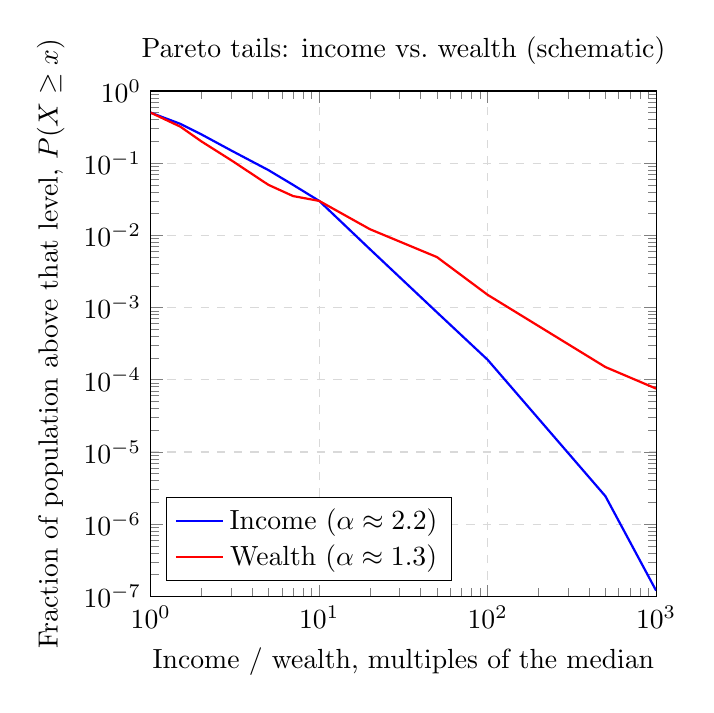
\begin{tikzpicture}
\begin{loglogaxis}[
    width=8cm, height=8cm,
    xlabel={Income / wealth, multiples of the median},
    ylabel={Fraction of population above that level, $P(X \geq x)$},
    xmin=1, xmax=1000,
    ymin=0.0000001, ymax=1,
    grid=major,
    grid style={dashed, gray!30},
    legend pos=south west,
    title={Pareto tails: income vs.\ wealth (schematic)},
]

% Income: body curves, then straight Pareto tail (alpha ~ 2.2)
\addplot[thick, color=blue, mark=none] coordinates {
    (1,    0.50)
    (1.5,  0.35)
    (2,    0.25)
    (3,    0.15)
    (5,    0.08)
    (7,    0.05)
    (10,   0.03)
    (20,   0.00644)
    (50,   0.000859)
    (100,  0.000189)
    (500,  0.00000244)
    (1000, 0.00000012)
};
\addlegendentry{Income ($\alpha \approx 2.2$)}

% Wealth: same body region, much flatter tail (alpha ~ 1.3)
\addplot[thick, color=red, mark=none] coordinates {
    (1,    0.50)
    (1.5,  0.32)
    (2,    0.20)
    (3,    0.11)
    (5,    0.05)
    (7,    0.035)
    (10,   0.03)
    (20,   0.01217)
    (50,   0.00500)
    (100,  0.00150)
    (500,  0.00015)
    (1000, 0.0000754)
};
\addlegendentry{Wealth ($\alpha \approx 1.3$)}

\end{loglogaxis}
\end{tikzpicture}
\end{document}